Grid-based spatial indexing is a well known algorithm in computer science, especially computer graphics, that allows for efficient lookup based on geometric criteria and also provides fast collision detection \cite{bentley1979data}.
Critical to the present application, it allows constant time retrieval of a superset of atoms guaranteed to contain all atoms within a given Euclidean distance.
%describe when/how you set the Euclidean distance cutoff
In our implementation, the bounding box of the protein and its symmetric copies is subdivided along each of the orthogonal axes to form grid boxes or cells.
A simple convention for handling atoms that are positioned along cell boundaries guarantees that each atom is hashed to a unique cell.
For a single dimension, $d$, the cell index, or hash, of a point $p$ is 
\begin{equation}
i_{d}(p) = int\left(N * \frac{p_{d} - min_{d}(P)}{max_{d}(P) - min_{d}(P)}\right)
\end{equation}

where $min_d(P)$ and $max_d(P)$ are the minimum and maximum coordinates in dimension $d$ over the set of points $P$, $N$ is the number of cells in dimension $d$, and $p_{d}$ is the coordinate of $p$ in $d$.
Following the same procedure in each dimension gives a unique cell location for every atom.
In this way, at the beginning of the simulation, each atom is assigned to a specific cell, or grid box.
A list of the atoms in each grid box is then maintained over the course of the simulation.
When computing the electrostatic contribution to solvent free energy of an atom, $a$, it is only necessary to loop over the atoms contained in boxes that intersect the sphere corresponding to the distance cutoff around atom $a$. 
Beyond that cutoff, charge effects are considered to be negligible \cite{gallicchio2004agbnp}.
See figure \ref{figure:grid_hash} for an illustration of grid based spatial indexing in two dimensions.

In the present implementation, cell size is at first set to 2.745 angstroms, and the number of cells in a given dimension depends on the "length" of the system in that dimension.
If the number of cells that this would require is unmanageably large, cells are then grown simultaneously in all dimensions such that the cell size is 1/250th of the longest dimension of the structure.

% cells figure, pretty
\begin{figure}[h]
\begin{center}
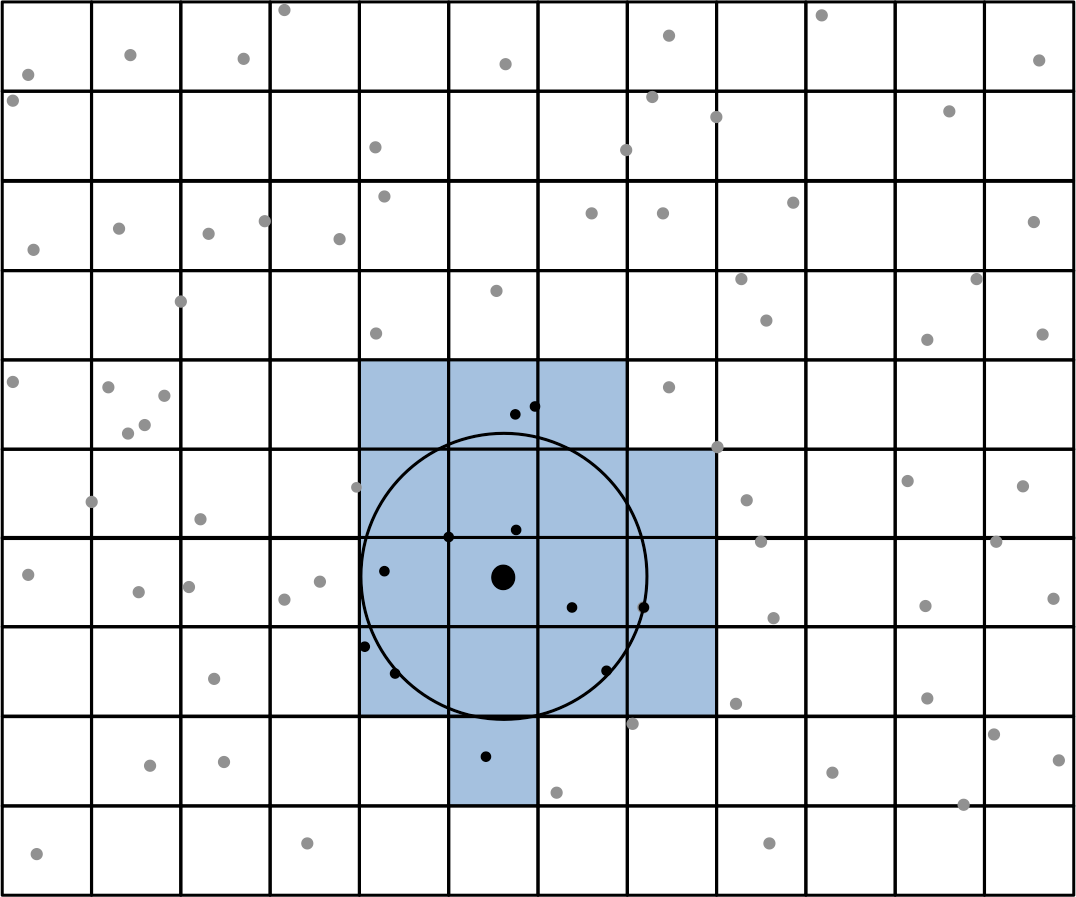
\includegraphics[width=0.6\textwidth]{figures/grid4_crop.png}
\caption{This illustrates, in two dimensions, the grid based spatial indexing method.
The naive S-GB method would require a distance computation to every other atom in the system.
By only considering atoms in cells intersecting the radius of influence, represented here in blue, it is possible to consider far fewer interactions.
Although only atoms inside the circle in this illustration contribute to surface charge, it is necessary to compute the distance over all black points.
Without using this hashing scheme, it would be necessary to compute the distance to each gray point as well.}
\label{figure:grid_hash}
\end{center}
\end{figure}
